% You should title the file with a .tex extension (hw1.tex, for example)
\documentclass[a4paper, 11pt]{article}

\usepackage{amsmath}
\usepackage{amssymb}
\usepackage{fancyhdr}
\usepackage{graphicx}
\usepackage{scribe}
\usepackage{graphicx}
\usepackage[margin=1in]{geometry}
\usepackage{graphicx}
\newcommand{\question}[2] {\vspace{.25in} \hrule\vspace{0.5em}
\noindent{\bf #1: #2} \vspace{0.5em}
\hrule \vspace{.10in}}
\renewcommand{\part}[1] {\vspace{.10in} {\bf (#1)}}

\newcommand{\myname}{Kriangsak Thuiprakhon}
\newcommand{\myemail}{kriangsak.thi@student.mahidol.edu}
\newcommand{\myhwnum}{}

\setlength{\parindent}{0pt}
\setlength{\parskip}{5pt plus 1pt}
 


\begin{document}

\medskip                        % Skip a "medium" amount of space
                                % (latex determines what medium is)
                                % Also try: \bigskip, \littleskip

\thispagestyle{plain}
\begin{center}                  % Center the following lines
{\Large ICCS481: Final Exam } \\
\myname \\
\myemail \\
\end{center}
\question{1: Random Walks}{}  In class, the cover time of an undirected, simple graph $G = (V, E)$ was shown to be at most $2|E|(|V| − 1)$. To test whether $u$ and $v $ are connected, the following algorithm is a weird one:
Start a random walk at $u$. \\

Perform a random walk for $T$ steps. If we visit v during this time, return "yes"; otherwise, "no”.

Find a setting of $T$ that ensures the algorithm will succeed with probability at least 1/2. Prove that your choice of $T$ provides the desired guarantee.

\textsc{solution}  
\begin{claim}
There exists a setting that performs a random walk of length $2n^3$, which is $T$ in the question, which allows for the  connectivity test of nodes  $u$ and $v$ on $G = (V, E)$ w.p. at least 1/2 it returns the correct answer
\end{claim}
 A simple pseudo codes is the following:
\begin{itemize}
\item Pick vertex $v = s \in_R G(V,E)$
\item Perform a random walk of T = $2n^3$ steps 
\item If   $v = t$, break and return "yes"
\item  Else, let draw  $v \in_R \{ w: (v,w) \in E\}$ 
\item If after T steps performed, $t$ has not been visited, then return "no"
\end{itemize}

\begin{proof}
To prove this, we need to find that the probability that the algorithm returns the incorrect answer: i.e., returns "no" when it is a "yes". From what is proven in class, the cover time  of an undirected graph is at most $2|E|(|V| − 1)$. we will new a bit more tools to prove this claim. In general, proved are available online, a simple, undirected  graph, has at most $O(n^2)$ edges.  
\begin{proof}
An edge is uniquely determined by its set of endpoints, which is a subset of the set of vertices of size 2, that is ${ n} \choose {2}$ or $O(n^2)$. 
\end{proof}
We will need also this lemma 
\begin{lemma}
 The effective resistance between any two nodes u and v is at most the length of the shortest path between them in G.
 \end{lemma}
 \begin{proof}
 The effective resistance between any two nodes $u$ and $v$ is the voltage difference  between $u$ and $v$ when
one ampere is injected into $u$ and removed from $v$. Let $p_1$ be the shortest path between $u$ and $v$. If $p_1$ is the only
path between $u$ and $v$, then, since $V =  IR$and $ R = \sum_{ i \in p_1} R_i $ we have that $\H{u,v} $ equals to the length of the shortest path. If there exists a second path $p_2$. Then the length of $p_2 \geq $the length of $p_1$. Therefore the resistance of $p_2$ is
greater than the resistance of $p_1$. Since $\frac{1}{R} = \frac{1}{R_1} + \frac{1}{R_2}$ , we know the resistance is less than the resistance on the 
shortest path. Therefore the effective resistance between u and v is less the one when there exists only one path between u and v. Hence the effective resistance between any two nodes is at most the length of the shortest path between them. 
\end{proof}
and the following definition,
\begin{definition}
Diameter of G: the maximum of all of lengths of the shortest path between any 2 vertices in G.
\end{definition}
we can now find the upper bound of the commute time , $C_{u,v}$ in a connected graph which we proved in the lecture that, for any connected graph, 
\begin{align*}
C_{u,v} &= 2mR_{eff}( u \sim v)\\
&= 2\times n^2 \times (n-1) && \textmd{ since the diameter of G is n-1} \\ 
& \leq 2n^3\\
\textmd{ Note that } H_{u,v} \leq  n^3
\end{align*}

we are now ready to prove our claim: we want to find with what probability that the algorithm returns an incorrect answer given the algorithm performs a random walk of length $2n^3$. By Markov's Inequality, we have that:
\begin{align*}
 Pr[ X > T  = 2n^3] &\leq \frac{\mathbb{E}[X] = H_{u,v}  }{2n^3} \\
 &\leq \frac{n^3}{2n^3} \\
 &\leq 1/2
\end{align*}
Therefore, given T = $2n^3$, the probability that the algorithm returns the correct answer is at least 1/2.
\end{proof}
%%
\question{2: Triangle Count Estimation}{}
\begin{itemize}
\item[(i)] Prove that if 

$$
\mathbb{E}[\alpha] = \frac{ 3  \tau}{m(n-2)}
$$
\begin{proof}
where $\tau$ is the total number of triangles in G. 
Notice that since $\alpha$ is an indicator random variable, it follows that
$$ \mathbb{E}[\alpha] = \P(w \sim \{u,v\}) \quad \quad  \forall w \in_R G \setminus \{u,v\}  $$
\begin{claim}

Let $w^*$ be a triangle in a graph G.  The probability that $w = w^*$ (i.e., $w$ is incident on $u$ and $v$, is given by
$$
Pr[ w= w^*] = \frac{1}{m(n-2)}
$$
\end{claim}

\begin{proof}
Please allow me to refer (copy) your proof in the paper.

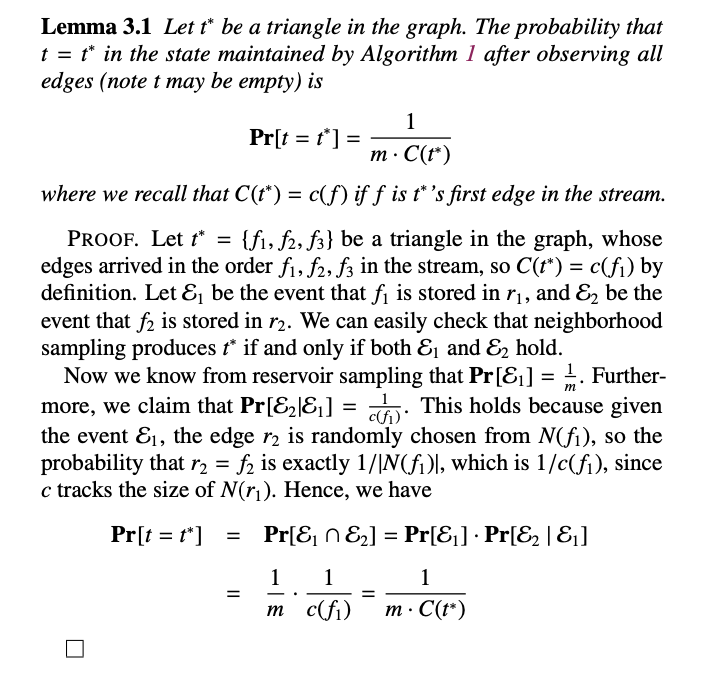
\includegraphics[width=\textwidth]{triangle.png}

in this case, I assume we treat $c(f_1)$ to be $n-2$ so it gives the probability $Pr[ w= w^*] = \frac{1}{m(n-2)}$
\end{proof}


Finally, we know that there can be 3 permutations  of edges for each of the triangle. This then yields the expectation of $\alpha$-estimator for a graph with $\tau$ triangles as follows:
$$
\mathbb{E}[\alpha] = \frac{ 3  \tau}{m(n-2)}
$$
\end{proof}
 \item[(ii)] Show that if $\hat{\alpha}  = \frac{1}{T} ( \sum_{i =1}^T \alpha_i)$ and $\hat{\tau} = \frac{m(n-2)}{3} \hat{\alpha}$ then, $\mathbb{E}[\hat{\tau}] = \tau$
 
 \begin{proof}
 The expectation of $\hat{\tau} $  can be computed as follows:
 \begin{align*}
\mathbb{E}[ \hat{\tau}] &=  \mathbb{E} \left[ \frac{m(n-2)}{3}  \frac{1}{T}  \sum_{i =1}^T \alpha_i \right]\\
&= \frac{m(n-2)}{3}  \frac{1}{T} \sum_{i =1}^T \mathbb{E}[ \alpha_i]  &&\textmd{ by linearity of expectation}\\
& = \frac{m(n-2)}{3} \cdot \frac{1}{T} \cdot T \cdot \frac{ 3 \tau}{m(n-2)} && \textmd{  by (i)}\\
& = \tau
 \end{align*}
 \end{proof}
 
 \item[(iii)] Let $\varepsilon \geq 0$ and $ 0 \leq \delta \leq 1/2$. Using is scheme, how large does $T$ have to be in order for $\hat{\tau}$ to satisfy $\Pr[|\hat{\tau} -\tau|] < \varepsilon] \geq 1 - \delta$?\\
 
 From our scheme, notice that our $\alpha$-estimators do not necessarily fall in the range [0,1]. Therefore, a rescaling is needed for Chernoff's bounds to apply. \\
 \textsc{From CALGO import A1.5, hehe :P: Rescaling Tricks.} \\

With $\mathbb{\hat{\tau}} = \tau$ from (ii), Assume $\tau_i \in [a,b] \text{ for } a \leq b \in \mathbb{R}$. Rescaling this random variable to be in [0,1] will allows Chernoff-Hoffding bounds to apply. 
Here is how we do it,
\begin{align*}
&a \leq \tau_i \leq b\\
& 0 \leq \tau_i -a \leq b-a \\
& 0\leq \frac{\tau_i -a}{b-a} \leq 1\\
\end{align*}
Let $Y_i$ denote $\frac{\tau_i -a}{b-a} $ now that $Y_i \in [0,1]$, we can find the expectation of $Y_i$
$$\mathbb{E}[Y] = \mathbb{E} [\frac{\tau -a}{b-a}] = \frac{\mathbb{E}[\tau] -na}{b-a} $$
Apply Chernoff-Hoffding bounds,\\
We need to show,
\begin{itemize}
\item For all $ t > 0$,\\
$$\Pr[\tau>\mu +t] \text{and} \Pr[\tau<\mu -t] \leq \text{exp}\{-2t^2n\}$$
\quad 
With Out Loss Of Generality, we can rewrite the probability to be,
\begin{align*}
&\Pr[\underbrace{\sum_{i=1}^n\frac{\tau_i -a}{b-a} }_{Y} > \underbrace{\frac{\mathbb{E}[\tau_i] -a}{b-a}}_{\mathbb{E} [Y]} + t ] \\
&\Pr[\sum_{i=1}^n \tau_i > \mathbb{E}[\tau] + \underbrace{(b-a)t}_{t'} ]\\
So, t = t'/(b-a)\\
&\therefore \Pr[\sum_{i=1}^n \tau_i > \mathbb{E}[\tau] + t] \leq exp\{-2(\frac{t'^2}{n(b-a)^2})\} 
\end{align*}
\end{itemize}
 
Next,  \textsc{From CALGO import A1.7 : Simple Samplers}
we now need to show that 

\begin{align*}
\Pr[|\hat{\tau} -\tau|] < \varepsilon]& \geq 1 - \delta \\
&\leq 1 - (Pr[ \hat{\tau} < \tau-\varepsilon ] +Pr[ \hat{\tau} > \tau+\varepsilon ])\\
&\leq 1 - 2(\underbrace{Pr[ \hat{\tau} < \tau-\varepsilon ]}_{*}) &&\text{ by symmetry}\\
\end{align*}

However, in *, $\hat{\tau}$ is given to be an empirical mean, with $1/T$ multiplied to the summation, we need to do a bit of manipulation in order for Chernoff-Hoffding bounds to apply. We rewrite the equation * to be,
\begin{align*}
Pr[ T\hat{\tau} < \underbrace{T\tau}_{**}-T\varepsilon ] & \leq exp\{-2(\frac{T^2\varepsilon'^2}{T(b-a)^2})\}  && \textmd{ by rescaling trick}\\
&\leq  exp\{-2(\frac{T\varepsilon'^2}{(b-a)^2})\} 
\end{align*}
** is $\mathbb{E}[\hat{\tau}]$ by linearity of expectation, which actually ready when we multiply the equation by N\\
Now we have the value of stars, plug it back into the equation, we have
\begin{align*}
Pr[[\hat{\tau}-\tau] \leq \varepsilon ] &\leq 1-\delta\\
&\leq 1 - \underbrace{2(exp\{-2(\frac{T\varepsilon'^2}{(b-a)^2})\} )}_{\delta} \\
\end{align*}
we can then derive $T$ as a function of $\delta$ and $\varepsilon$ 

$$\delta = 2(exp\{-2(\frac{T\varepsilon'^2}{(b-a)^2})\} )
\Leftrightarrow
T =  \frac{(b-a)^2}{-2 \varepsilon'^2} \ln (\delta/2)$$
I know it smells like  something is wrong in (hopefully only)  the last part... But MY brain is already dead. :(

\end{itemize}
\end{document}
